\label{capitolo2}
\section{Principi di modellazione}
I classici problemi di controllo sono divisi in "processi" e "motion" ma noi ci occuperemo principalmente dei primi. Incontreremo in oltre alcune PDE (Equazioni differenziali parziali) ma con al massimo una coordinata spaziale (tubi). In altri casi invece ci imbatteremo in sistemi di equazioni differenziali ordinarie ricavate dalla manipolazione di equazioni spaziali discrete ricavate da un approccio a volumi finiti (FV).\\
I tre aspetti principali dei quali ci occuperemo saranno sistemi di tipo idraulico, elettrico o termico; alcuni problemi di tipo meccanico si presenteranno ma solo sporadicamente e considereranno una sola coordinata spaziale.
\subsection{Sistemi termo-idraulici}
Le equazioni che incontreremo sono scritte facendo riferimento a un volume di controllo, non necessariamente costante, considerando un solo liquido incomprimibile.
\subsubsection{Equazione di bilancio delle masse}
L'equazione \ref{bmass} rappresenta l'equazione di bilancio delle masse dove $M$ è la massa di liquido contenuta nel volume di controllo, $w_i$ è il flusso che entra (se positivo) o esce (se negativo) dal volume di controllo.
\begin{equation}
\label{bmass}
\frac{dM(t)}{dt}=\sum_{i=1}^{n_m}w_i(t)
\end{equation}
\subsubsection{Equazione di bilancio dell'energia}
Le equazioni di bilancio dinamico che riguardano l'energia considerano un volume di controllo nel quale è contenuta tutta l'energia $E$ e dove $n_m$ flussi di massa e $n_h$ potenze termiche $Q_j$ entrano (escono se negativi).\\
Ovviamente la derivata dell'energia $E$ è la somma dei vari flussi termici ai quali non è associato alcun trasferimento di massa.\\
La derivata temporale dell'energia è data da due contributi coesistenti:
\begin{itemize}
\item apporti di energia legati al trasporto di massa dati da:
$$Portata \times Energia_-specifica_-del_-fluido$$
\item lavoro eseguito dal flusso entrante o uscente sul volume di liquido espresso in forma differenziale come:
$$dL=d(pv)=d(p/\rho)$$ o anche come $$dL=pdv+vdp$$
\end{itemize}
Dove la componente $pdv$ è detta "lavoro di compressione" e $vdp$ è il "lavoro di pulsione".
La grandezza che esprime l'apporto di energia di una portata di fluido entrante è data dalla \ref{entspec} che esprime l'entalpia specifica del fluido.
\begin{equation}
\label{entspec}
h=e+\frac{p}{\rho}
\end{equation}
Dove $e$ indica l'energia interna specifica.\\
Pertanto l'equazione di conservazione dell'energia è data dalla \ref{ener}
\begin{equation}
\label{ener}
\frac{dE(t)}{dt}=\sum_{i=1}^Nw_i(t)h_i(t)+\sum_{j=1}^MQ_j(t)
\end{equation}
Il termine $e$ domina (negli esempi ed esercizi di questo corso) di molto il termine $p/\rho$ in questo caso si può considerare l'entalpia e l'energia interna uguali e pari a $cT$ dove c è il calore specifico.
Detto ciò, tenendo conto delle nostre ipotesi e delle semplificazioni fatte, la formula del bilancio di energia si semplifica come nella \ref{bener}.
\begin{equation}
\label{bener}
c\frac{dM(t)T(t)}{dt}=c\sum_{i=1}^{n_m}w_i(t)T_i(t)+\sum_{j=1}^{n_h}Q_j(t)
\end{equation}
Alcune volte la massa rimane costante allora $$cM\frac{T(t)}{dt}=c\sum_{i=1}^{n_m}w_i(t)T_i(t)+\sum_{j=1}^{n_h}Q_j(t)$$
In altri casi è conveniente espandere la derivata a sinistra e sottrare l'equazione di massa moltiplicata per cT.
$$
\begin{array}{ccccccc}
cM(t)\frac{dT(t)}{dt} & + & cT(t)\frac{dM(t)}{dt} & = & c\sum_{i=1}^{n_m}w_i(t)T_i(t) & + & \sum_{j=1}^{n_h}Q_j(t)\\
\\
&-&cT(t)\frac{dM(t)}{dt}& = &-cT(t)\sum_{i=1}^{n_m}w_i(t)&&\\
\\
\hline
\\
cM(t)\frac{dT(t)}{dt}& + && = &c\sum_{i=1}^{n_m}w_i(t)(T_i(t)-T(t))&+&\sum_{j=1}^{n_h}Q_j(t)\\

\end{array}
$$
L'equazione precedente è chiamata equazione "net energy".\\
\subsubsection{Equazione della quantità di moto}
Per quanto riguarda la quantità di moto l'equazione in questo corso è utilizzata per modellizzare le condutture.\\
In un tubo la derivata della quantità di moto  è uguale alla somma delle forze che agiscono su di esso:
\begin{itemize}
\item pressione ai capi della conduttura
\item forza di gravità
\item forze di atrito sulle superfici laterali
\end{itemize}
tutte riferite lungo l'ascissa x del tubo (sull'asse y le componenti sono a 90° o sono bilanciate da forze esterne)
\begin{figure}
\centering
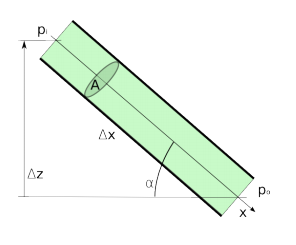
\includegraphics[width=5cm]{img/tubo.png}
\caption{Sezione di tubo\label{fig:tubo}}
\end{figure}
L'equazione dei momenti per il sistema in Fig. \ref{fig:tubo} è data dalla \ref{eqtubo} 
\begin{equation}
\label{eqtubo}
M\frac{du(t)}{dt}=A p_i(t)-A p_o(t)+ M g \sin(\alpha)-f_a(t)
\end{equation}
Dove $$f_a=K_f A_l\rho u|u|$$

La quantità $K_f$ è detta \emph{coefficente di frizione} e dipende dalle caratteristiche di contatto tra il fluido e le pareti. Inoltre la formula contiene un termine di inerzia che però nei nostri esempi non considereremo questo perchè i fenomeni idraulici sono molto più veloci delle costanti di tempo di quelli termici. Quindi la formula della quantità di moto si riduce alla \ref{qmoto}.
\begin{equation}
\label{qmoto}
A(p_i(t)-P_o(t))+Mg\frac{\Delta z}{\Delta x}-K_f A_l \rho u(t)|u(t)|=0
\end{equation}
Concludendo indicando con:
\begin{itemize}
\item A la sezione del tubo,
\item L la sua lunghezza
\item e $\omega $il suo perimetro interno
\end{itemize}
e ricordando che $w=\rho A u$ abbiamo che:
$$p_i-p_o= K_f\frac{\omega L}{\rho A^3} w|W|-\rho g\Delta z$$
L'equazione della quantità di moto può rappresentare il comportamento tipico di una valvola. Dal nostro punto di vista una valvola è come una piccola sezione variabile di tubo in cui $\Delta z =0$ e la velocità è data dalla formula seguente:
$$w=C_v\phi(x)\sqrt{\rho (p_i - p_o)}$$
dove $C_v$ è il coefficente di flusso e $\phi(x)$ è la caratteristica intrinseca della valvola.
\subsubsection{Equazione dell'energia nei corpi solidi}
Per quanto riguarda il caso in cui non vi sia scambio di massa (ad esempio conduzzione attraverso una parete) la formula diventa:
$$cM\frac{dT(t)}{dt}=\sum_{j=1}^{n_h}Q_j(t)$$
Nel caso in cui il muro non sia uniforme lo si divide in più livelli e si applica sempre la stessa formula.\\
\subsubsection{Equazioni dei flussi di calore}
Le equazioni per i flussi di calore ci servono per modellizzare tre fenomeni:
\begin{itemize}
\item Conduzione
\item Convezione
\item Irraggiamento
\end{itemize}
Per quanto riguarda la conduzione la potenza termica è data da :
$$Q_{ab}=G(T_a(t)-T_b(t))$$
Dove $T_a$ e $T_b$ sono le temperature ai due lati e G è:
$$G=\lambda \frac{A}{s}$$
con A la superfice s lo spessore e $\lambda$ la conduttività termica del materiale.\\
Nel caso di convezione la formula della potenza termica tra flusso e parete è data da:
$$Q_{wf}=\gamma A(T_w(t)-T_f(t))$$
\subsection{Sistemi elettrici}
Per quanto riguarda i sistemi elettrici saranno effettuate alcune semplificazioni per rendere più chiari ed intuitivi i concetti:
\begin{itemize}
\item una sola sincrona frequenza per tutta la rete.
\item tutti i generatori forniranno un voltaggio costante.
\item le linee di trasmissione avranno un comportamento lineare.
\item sistemi ad una fase
\end{itemize}
Inoltre adotteremo un sistema di modellizzazione basato sui fasori.\\
Ogni quantità che varia in modo sinusoidale a frequenza costante $\omega$ può essere rappresentata come segue:
$$A\cos(\omega t +\theta)= \Re(Ae^{j(\omega t+\theta)})=\Re(Ae^{j\theta}e^{j\omega t})$$
Dove il fasore $A^{j\theta}$ esprime la fase e l'ampiezza rispetto a un opportuno sistema di riferimento.
\subsubsection{La legge di Ohm}
$$\underline{V}=\underline{Z}\underline{I},\underline{I}=\underline{Y}\underline{V}$$
dove $\underline{V},\underline{I}$ sono rispettivamente i fasori che indicano voltaggio e corrente e $\underline{Z},\underline{Y}$ sono impedenza e ammettenza. Tipicamente le ultime due quantità vengono espresse come $\underline{Z}=R+iX$ e $\underline{Y}=G-iB$ dove $R,X,G,B$ sono rispettivamente la resistenza, la reattanza, la conduttanza e la suscettanza.\\
La potenza espressa in termini di fasori è data da:
$$S=V_{RMS}I^*_{RMS}=P+jQ=Ae^{j\phi}$$
dove possiamo distinguere una componente attiva:
$$P=\Re(S)=V_{RMS}I_{RMS}\cos \phi$$
e una componente reattiva:
$$Q=\Im(S)=V_{RMS}I_{RMS}\sin \phi$$
